\documentclass{article}

\usepackage[margin=1.0in]{geometry}
\usepackage{graphicx}
\usepackage{amsmath}
\usepackage{float}
\usepackage{enumitem}
\usepackage{gensymb}

\title{CSC 577 HW1}
\date{1/16/2019}
\author{Simon Swenson}

\begin{document}

\pagenumbering{gobble}
\maketitle
\pagenumbering{arabic}

\section{Introduction}

\begin{figure}[!ht]
	\centering
	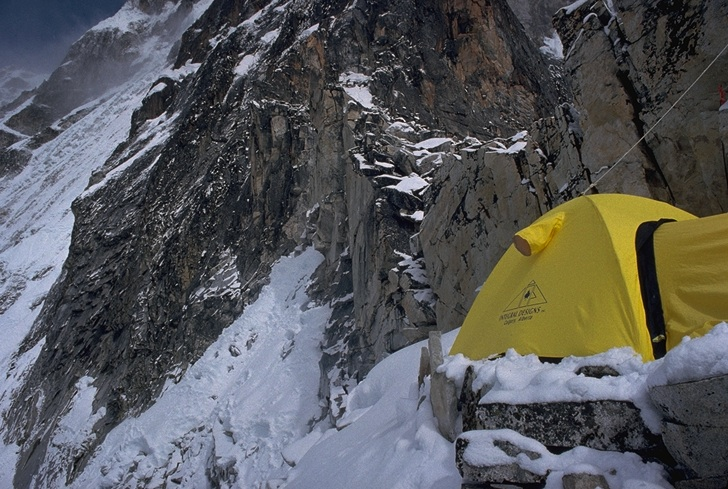
\includegraphics[width=120mm]{figs/tent.jpg}
	\caption{The original tent image, a key point of focus for this homework 
        assignment.}
\end{figure}

All homework problems (including grad problems) were completed. I had some 
MATLAB experience from Probablistic Graphical Models last semester, so this 
was not that time consuming, but it was a bit tedious, as I needed a refresher, 
and learning the syntax and features of any language is always a bit tedious.

\section{(\#6)Documentation for the Code of HA1}

Below is the output of "help ha1" which documents the functionality of the code 
used for this assignment:

--- help for hw1 ---

 hw1 Performs all commands needed for hw1.
    The return value is the number of completed homework questions. First, 
    hw1 reads in an image, displays it in a figure, then saves the
    image with the extension '.out.jpg'. Then, it displays statistics (min, 
    max) for each channel in the image. Then, the image is converted to a
    grayscale. This grayscale image is displayed as a figure. After that,
    each separate channel is taken as a grayscale image and displayed. To
    further experiment with channels, a new 3-channel image is produced
    which permutes the channels of the original image. To experiment with
    indexing, the grayscale image from earlier is modified so that each
    fifth pixel along the rows and columns are turned white. This is also
    displayed in a figure. In addition to the statistics gathered earlier,
    a histogram is then generated for each channel and shown in a figure.
    After that, to experiment with function plotting, the sin and cosine
    function are plotted from the domain -pi to pi. To experiment with
    matrix operations, an arbitrary matrix equation is solved by using
    inv, linsolve, and '\'. The topic of modifying certain pixel values in
    the grayscale image is then returned to, and a one-liner is used to
    perform a similar operation to the lattice operation that the nested 
    loop performed earlier. A similar method is then used to set all pixel
    values over a certain threshold to black. Finally, the function
    explores PCA and transforms a set of data points based on their PCA.

\section{(\#7) Basic Image Data Structures}

A cursory look at the image data after it has been loaded (by using the "whos" 
function) reveals that the image 
is stored as a three dimensional matrix/tensor with dimensions representing y 
coordinate, x coordinate, and channel (r, g, b), in that order. The size of the 
tensor is 489 x 728 x 3. All elements in that matrix/tensor are of type "uint8."
To hold onto that size information for future use, we can assign multiple 
variables at the same time, since "size" returns an n-tuple.

In addition to the dimensions of the image, other useful statistics can be 
gathered. For example, by using "min" and "max," we find that the minimum and maximum values 
are as follows:

\begin{itemize}
    \item Minimum of red = 0
    \item Minimum of green = 0
    \item Minimum of blue = 0
    \item Maximum of red = 251
    \item Maximum of green = 248
    \item Maximum of blue = 253
\end{itemize} 

At first, I was 
surprised at the minimum findings, as images usually do not contain true black. 
However, this finding does not necessarily mean that there is a (0, 0, 0) pixel 
in the image, just that 0 appears for each channel in at least one pixel, not 
necessarily the same pixel for all three channels.

Finally, the image was converted to a grayscale image. This created a great 
point of comparison for the following task, which examined each individual 
channel in the image \textit{as if it were a grayscale image}.

\section{(\#8) Image Channels}

For this experiment, each channel of the image was converted to a grayscale 
image separately. This really illustrated the effect of each channel on the 
image, especially the tent. However, much of the image is desaturated, which 
made it a bit harder to draw findings from this experiment.

\begin{figure}[!ht]
	\centering
	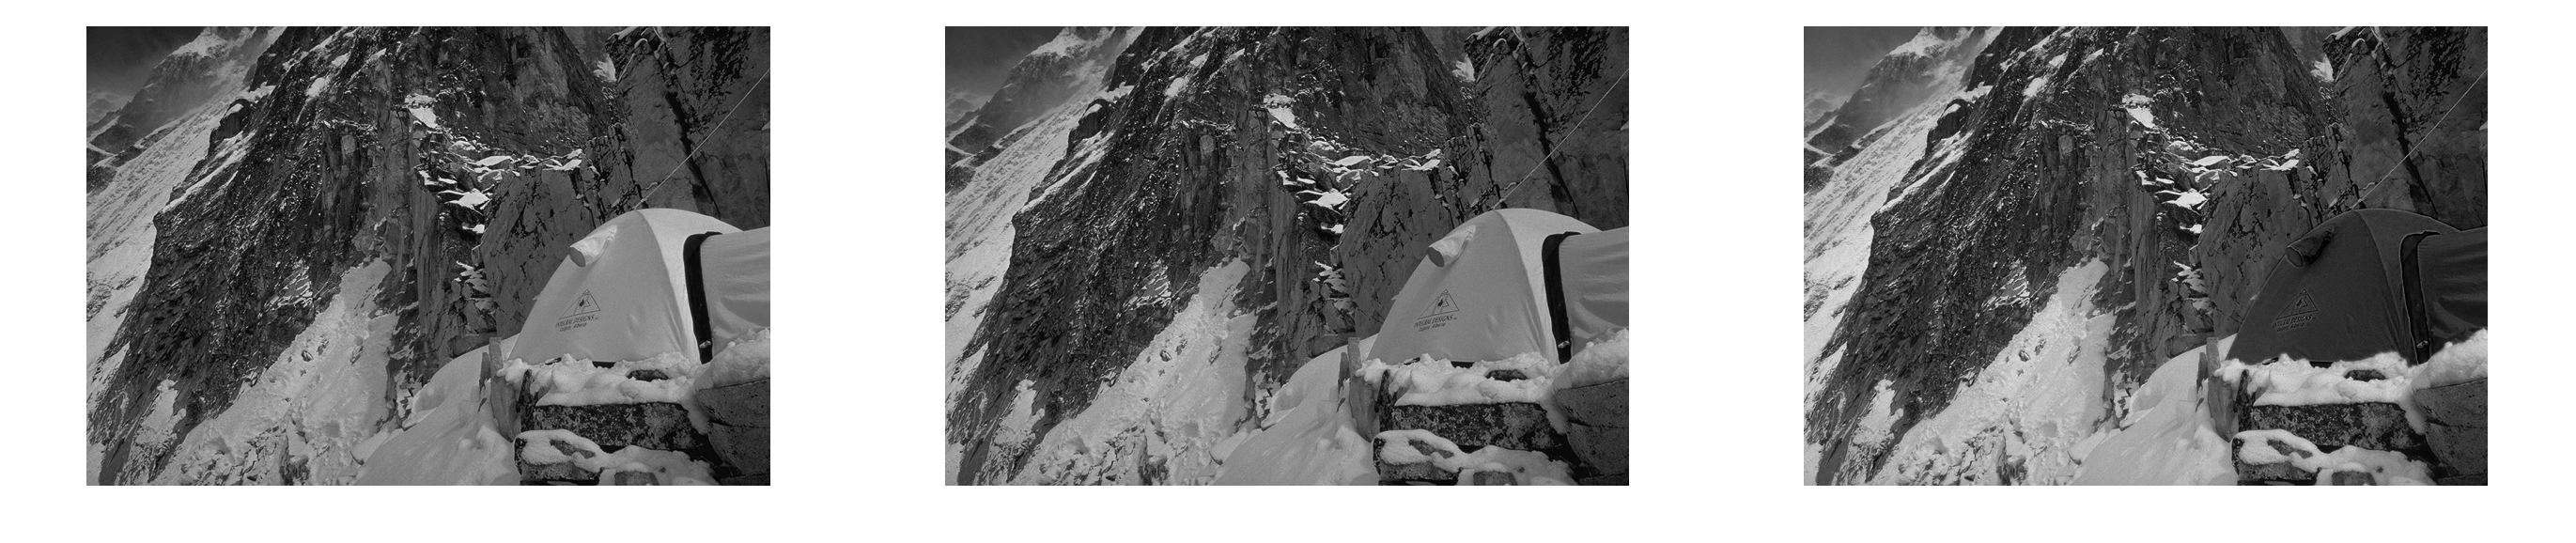
\includegraphics[width=160mm]{figs/tent_channel_comparison.png}
	\caption{Each channel of the original image, represented separately as if 
        they were grayscale. Left: red channel, center: green channel, right: blue 
        channel.}
\end{figure}

The most striking difference between the three channels is the amount of red and 
green in the tent when compared to the amount of blue. This illustrates that 
yellow can be reproduced for human eyes by simply combining equal amounts of 
red and green light. As the yellow in the image is so saturated, very little 
blue is present, but, as we can see in the desaturated rock cliffs and snow, 
as colors get closer to gray, each channel starts to have an equal "say" in the 
final value. One final note, which may seem a bit obvious, is that white is 
reflected by a high value for each of the three channels, and black si reflected 
by a low value for each of the three channels.

Another interesting experiment involving the color channels of the image is to 
simply permute the channels and display the resulting color image. The most 
important thing this reveals is that a large red value and a large blue value 
create purple, as can be seen in the purple tent.

\begin{figure}[!ht]
	\centering
	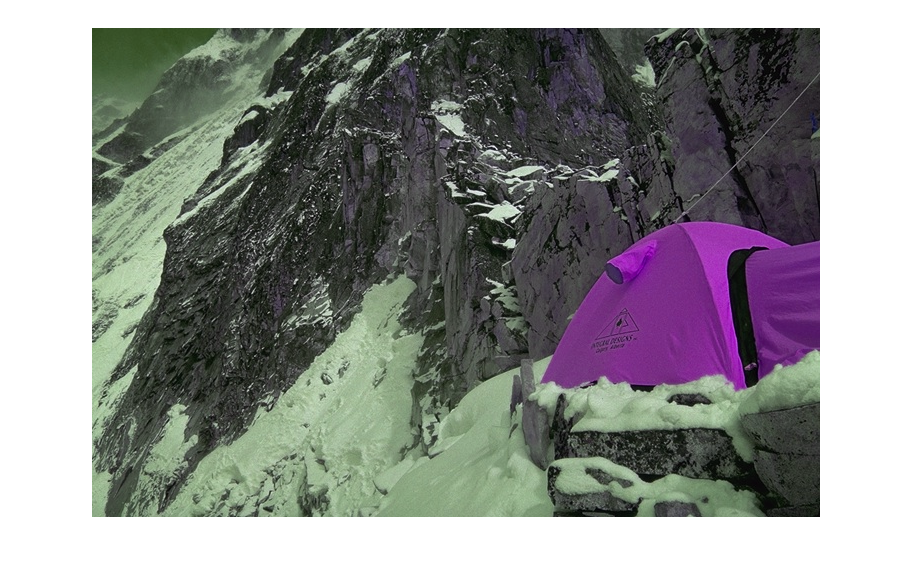
\includegraphics[width=120mm]{figs/tent_permuted_channels.png}
	\caption{A new image created by permuting the channels of the original tent 
        image. In this image, green was moved to red, blue was moved to green, and red 
        was moved to blue. This reveals that a high red and a high blue value produce 
        purple.}
\end{figure}

\section{(\#9) Manipulating Matrices}

MATLAB, as its name suggests, is an extremely useful tool for dealing with 
matrices. Thus, the various matrix operations are important to learn. For this 
experiment, we used a for loop to address every fifth pixel of the grayscale 
image, both horizontally 
and vertically, and turn it white. The results follow in two different formats.

\begin{figure}[!ht]
	\centering
	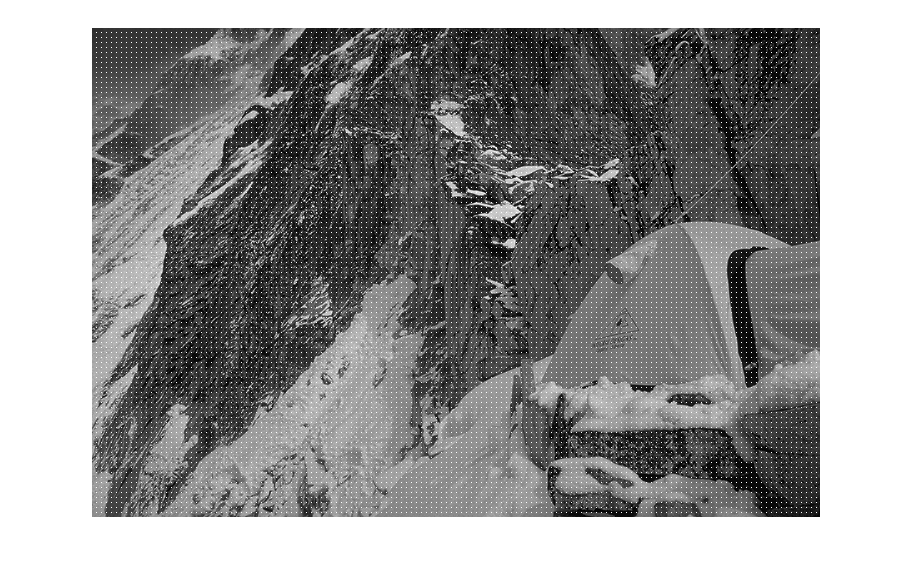
\includegraphics[width=120mm]{figs/tent_white_dots.png}
	\caption{The resulting lattice of white dots when shown using the "imshow" 
        function.}
\end{figure}

\begin{figure}[!ht]
	\centering
	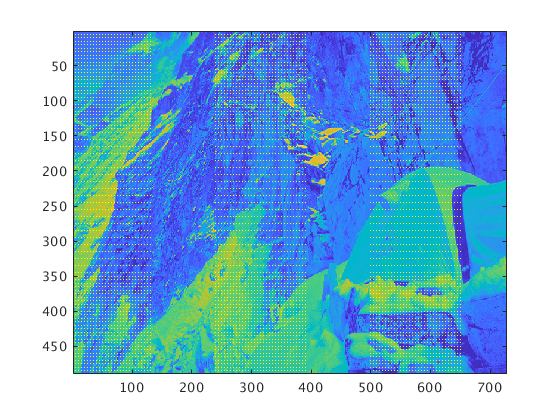
\includegraphics[width=120mm]{figs/tent_white_dots_imagesc.png}
	\caption{The resulting lattice of dots when shown using the "imagesc" 
        function.}
\end{figure}

The two display modes of the data have their strengths and weaknesses. To view 
the image as it actually is, "imshow" is the obvious choice. It displays 2 
dimensional matrices as gray images and 3 dimensional tensors as color images. 
This corresponds very nicely with the output from "imread." However, the second 
display method could be fruitful for visualizing data which does not 
necessarily correspond to the wavelengths of light we can normally see. For 
example, a similar hue-based heatmap approach is used in infrared cameras to 
visualize radiant heat. In this case, however, I think the best visualization 
is the grayscale image, as the backing data is derived from wavelengths that we 
can actually see. In addition, the small white pixels are harder to see when 
the image is squished as it is in "imagesc."

\section{(\#10) Histograms}

While the min and max values of each channel above are a good start for 
understanding the image, there are more robust statistics that we can use. 
Histograms give us a good overview of the \textit{concentration} of various 
color values 
for each of the three channels.

\begin{figure}[!ht]
	\centering
	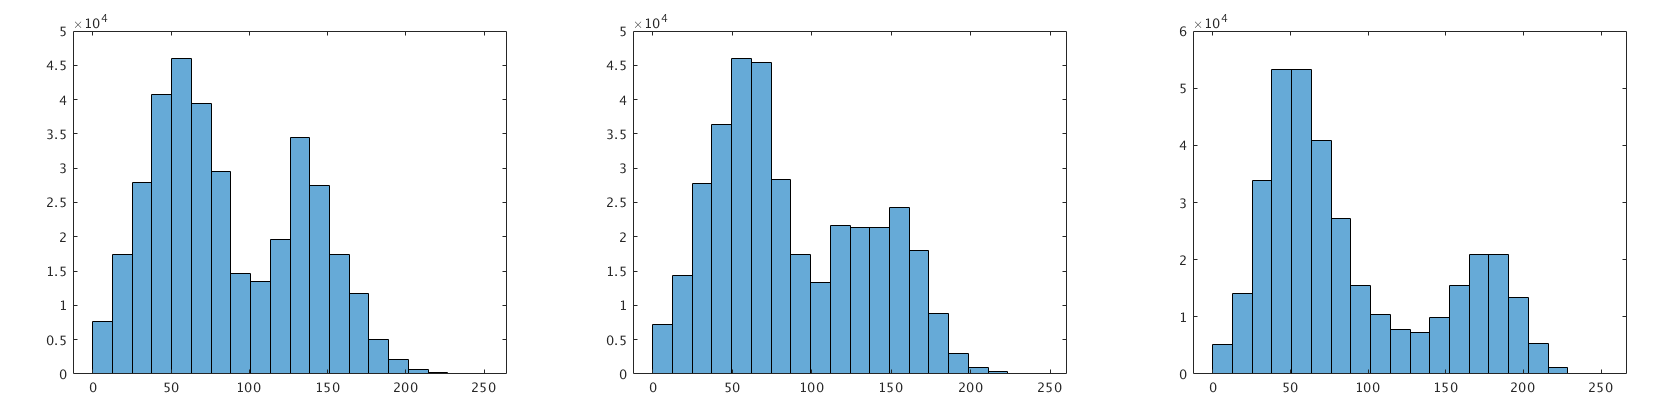
\includegraphics[width=160mm]{figs/hist_all.png}
	\caption{Three histograms, each representing the concentration of values for 
        a given channel. Left: red, center: green, right: blue.}
\end{figure}

The histogram is acually very reflective of the broad regions of the image. This 
image is very simple, and has three broad regions: cliffs, the tent, and snow. 
All three histograms show a very large hump near 50, reflecting the large area 
of cliffs in the image. The tent and snow are a little harder to tease apart. 
Comparing the red histogram to the blue histogram gives us some hints, however. 
The peak of the blue hump is at around 175. To me, this indicates that the peaks 
for the snow will be at 175 for the other two channels. However, the peaks for 
red and green are actually closer to 130-150. This is due to the tent. This 
illustrates one weakness of histograms: if two regions of the image have colors 
that are close in value to one another, you will not necessarily be able to 
distinguish those regions in the histogram.

\section{(\#11) Plotting}

The following is a very simple plot to get used to how plotting is done in 
MATLAB.

\begin{figure}[!ht]
	\centering
	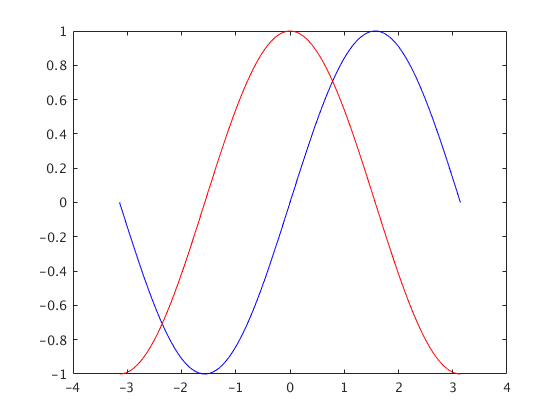
\includegraphics[width=120mm]{figs/sin_cos.png}
	\caption{The plots of sin (blue) and cosine (red) from -pi to pi.}
\end{figure}

\section{(\#12) Playing with Linear Algebra}

A good grasp of linear algebra is necessary for success in this course. Luckily, 
MATLAB has good builtin functions for performing common linear algebra tasks. 
This experiment involved using those builtins to solve for $x$ in a system of 
linear equations of the form $Ax = y$. The matrix can be represented as:

$$
\begin{bmatrix}
3 &  4 &  1 \\
2 & -1 &  2 \\
1 &  1 & -1
\end{bmatrix} x = \begin{bmatrix}
9 \\
8 \\
0
\end{bmatrix}
$$

To solve this equation, $x$ must be isolated. Thus, the matrix $A$ must be 
inverted. MATLAB has a number of methods to do so: "inv," "linsolve," and the 
"\\" operator.

The answer using "inv" was:

$$
x = \begin{bmatrix}
\sim 1.9375 \\
\sim 0.2500 \\
\sim 2.1875
\end{bmatrix}
$$

To verify this, we plug it into the original equation and perform matrix 
multiplication, which yields:

$$
\begin{bmatrix}
3 &  4 &  1 \\
2 & -1 &  2 \\
1 &  1 & -1
\end{bmatrix} \begin{bmatrix}
\sim 1.9375 \\
\sim 0.2500 \\
\sim 2.1875
\end{bmatrix} = \begin{bmatrix}
9 \\
8 \\
0
\end{bmatrix}
$$

An interesting side-effect of using floating point arithmetic for this task is 
that answers are not usually exact. This would be possible with arbitrary 
precision arithmetic, but, often, computer hardware, especially GPUs, is much 
faster at 
performing floating point operations than operations on arbitrarily large 
numbers. Comparing the answer above with the answer provided by linsolve, we 
see that they are not exactly the same. In fact, the difference between them is: 

$$
1.0 \times 10^{-15}
\begin{bmatrix}
\sim 0.2220 \\
\sim -0.0278 \\
0
\end{bmatrix}
$$

This could be the result of doing the operation in two steps by first inverting 
$A$, then multiplying $A^{-1} y$, which could cause cascading error, whereas
 "linsolve" might be optimizing in 
some other way. However, the error value is negligible, in this case.

\section{(\#15) Matrix Manipulations Without Explicit Loops}

Earlier, we explored using a nested for loop to index particular (x, y) 
coordinates of the image. However, this task can be done much more simply by 
using a conditional within the index expression. This will result in only 
indices which meet the condition being used. This is similar to a feature in 
python's pandas library, and the syntax is very similar. This MATLAB feature was 
used to produce the following two figures:

\begin{figure}[!ht]
	\centering
	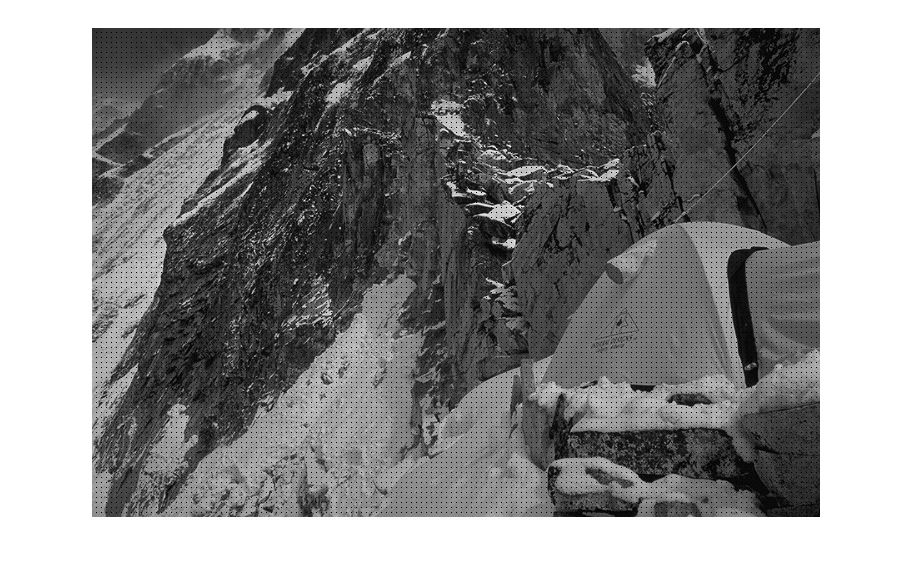
\includegraphics[width=120mm]{figs/tent_black_dots.png}
	\caption{Here, we use conditionals within the index expression to address 
        every fifth x and y, then set its color to black.}
\end{figure}

\begin{figure}[!ht]
	\centering
	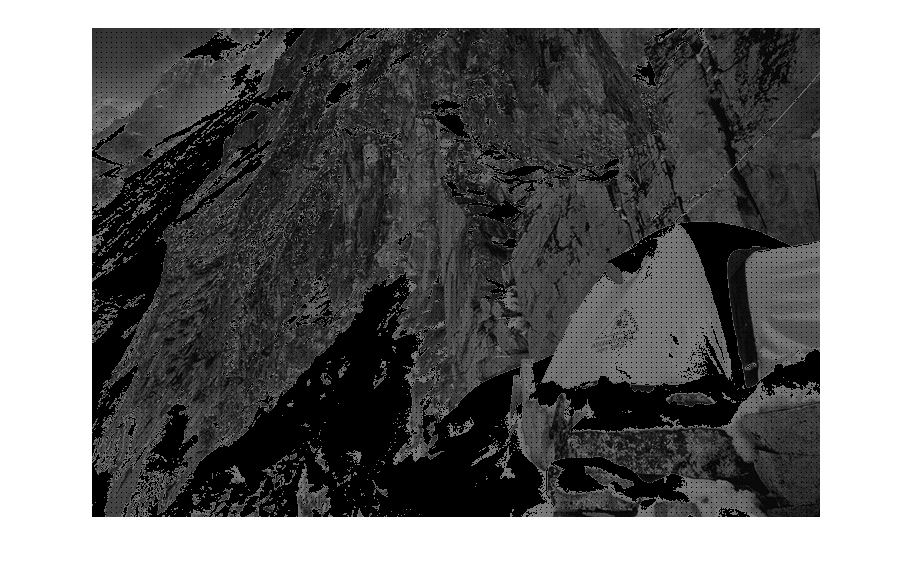
\includegraphics[width=120mm]{figs/tent_threshold.png}
	\caption{After setting each fifth x and y to black, a similar expression was 
        used to address pixels with a value over a certain threshold, then set 
        the values of those pixels to black.}
\end{figure}

\section{(\#16) PCA}

We briefly studied PCA in my undergraduate linear algebra, but that was a while 
ago, so this review was welcome. An example dataset to which PCA will be applied 
is shown below:

\begin{figure}[!ht]
	\centering
	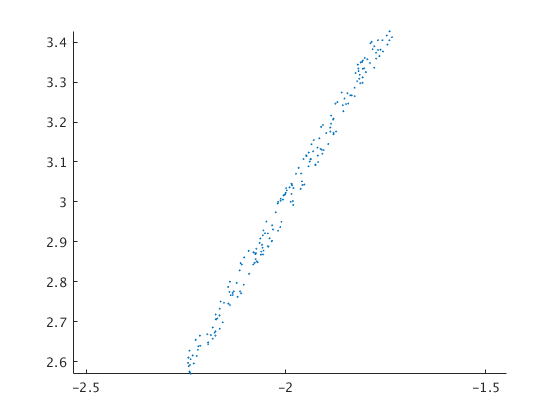
\includegraphics[width=120mm]{figs/pca_none.png}
	\caption{An example data set. Note that, it appears to have a very stark 
        cluster, but that cluster is not orthogonal to the axes. PCA attempts 
        to transform this dataset so that the principal components are 
        orthogonal to the axes. In this case, it means that a vector pointing to 
        the top-right will be the first principal component.}
\end{figure}

The corresponding covariance matrix is:

$$
C = \begin{bmatrix}
\sim 0.0211 & \sim 0.0356 \\
\sim 0.0356 & \sim 0.0608
\end{bmatrix}
$$

To me, it seems like this data could be represented much more naturally by 
rotating it either -60\degree or 30\degree so that the data varies substantially 
over only one axis rather than both axes. We could let the new basis vectors be 
something like:

$$
b_{1} = \begin{bmatrix}
\frac{1}{\sqrt{2}} \\
\frac{1}{\sqrt{2}}
\end{bmatrix}
$$

$$
b_{2} = \begin{bmatrix}
\frac{-1}{\sqrt{2}} \\
\frac{1}{\sqrt{2}}
\end{bmatrix}
$$

In this case, I would expect the covariance matrix to be diagonal and have a 
large value like 1 in the upper-left and a small value like 0.05 in the bottom-
right. This is because the first dimension would span a much larger range than 
the second dimension.

\section{(\#17) PCA II}

It turns out that the new basis vectors are actually the eigenvectors of the 
covariance matrix. Thus, we can use the "eig" builtin function. Doing so 
results in a matrix in which each column is one of those eigenvectors:

$$
E = \begin{bmatrix}
\sim 0.0211 & \sim 0.0356 \\
\sim 0.0356 & \sim 0.0608
\end{bmatrix}
$$

To verify that the eigenvectors are orthogonal, we can simply verify that their 
dot product is zero, which turns out to be true. Then, we can simply transform 
the data by multiplying the original data set with the eigenvector matrix on the 
right. This yields the following plot:

\begin{figure}[!ht]
	\centering
	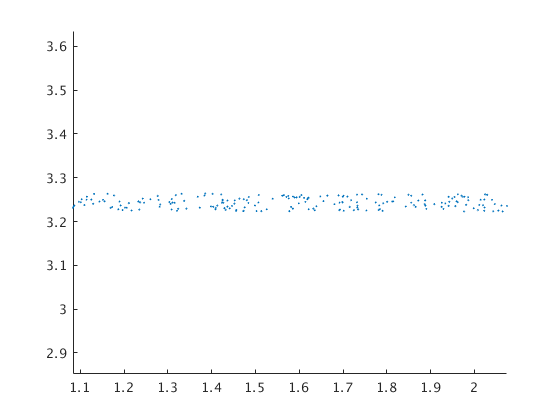
\includegraphics[width=120mm]{figs/pca_complete.png}
	\caption{A new coordinate system, transformed to the basis of the 
        eigenvectors. Note that the points are now essentially arranged 
        orthogonally to the x axis.}
\end{figure}

The resulting covariance matrix is diagonal, as we had hypothesized:

$$
C = \begin{bmatrix}
\sim 0.0818 & 0 \\
0 & \sim 0.0001
\end{bmatrix}
$$

The values that I had anticipated above were much different. I should have 
paid closer attention to the data range, which was less than one. This would 
yield a standard deviation of less than one, and thus a covariance even smaller 
still. However, the difference in magnitude of the two non-zero values in the 
covariance matrix was correctly postulated. One value is large and one is very 
small. Strikingly, the sums of the diagnals of the two covariance matrices 
(before transformation and after transformation) are the same. To me, this is 
unexpected, because the other values in the original covariance matrix seem 
to disappear. I would have expected those values to somehow get incorporated 
into the diagonals of the new covariance matrix, but that is probably a lack 
of understanding of what covariance really means.
\end{document}